\documentclass[12pt, addpoints, answers]{exam}
\usepackage[left=0.1in, right=0.1in, top=0.6in,bottom=0.1in]{geometry}
\usepackage{enumitem}
\usepackage{amsmath}
\usepackage{tikz}
\usepackage{ulem}
\usetikzlibrary{shapes.geometric, arrows.meta, positioning}

% --- Tikz set for diagram
\tikzset{
    box/.style={rectangle, draw, minimum width=1.8cm, minimum height=1cm, align=left, font=\small},
    doublebox/.style={rectangle, draw, double, double distance=1.5pt, minimum width=2.5cm, minimum height=1cm, align=left, font=\small},
    decision/.style={diamond, draw, minimum width=1cm, minimum height=1cm, align=center, aspect=2, font=\small},
    doubledecision/.style={diamond, double, draw, minimum width=1cm, minimum height=1cm, align=center, aspect=2, font=\small},
    attribute/.style={rectangle, draw, minimum width=1.5cm, minimum height=0.6cm, align=center, font=\small},
    arrow/.style={-Stealth, thick},
    doublearrow/.style={-Stealth, thick, double, double distance=1.5pt},
    dashedline/.style={thick, dashed},
    line/.style={thick},
    doubleline/.style={thick, double, double distance=1.5pt}
}

% --- Make choices use open circles instead of letters ---
\renewcommand{\choicelabel}{\raisebox{0.15ex}{$\bigcirc$}}

% Header/footer formatting
\pagestyle{headandfoot}
\runningheadrule
\firstpageheadrule
\firstpageheader{Database Management Systems}{Ch 7 Old}{Fall 2025}
\runningheader{}{Ch 7 Old}{}
\runningfooter{}{}{}

\begin{document}
\noindent Name:\ \makebox[3in]{\hrulefill}\hfill Points Scored: \underline{\hspace{3em}} / \numpoints
\begin{questions}

% ------------------ TRUE/FALSE SECTION ------------------
\section*{Part I — True/False}

\begin{minipage}{\linewidth}
\question[2]
True or False: In an Entity-Relationship model, it is possible for an attribute to be associated with a relationship set.\par\vspace{0.5em}
\begin{checkboxes}
    \CorrectChoice True
    \choice False
\end{checkboxes}
\end{minipage}\vspace{1em}

\begin{minipage}{\linewidth}
\question[2]
True or False: In a one-to-many relationship between entity sets X (one side) and Y (many side), where participation is optional for both entities, 
it is possible for there to be 3 objects of type X with no objects of type Y.\par\vspace{0.5em}
\begin{checkboxes}
    \CorrectChoice True
    \choice False
\end{checkboxes}
\end{minipage}\vspace{1em}

\begin{minipage}{\linewidth}
\question[2]
True or False: There are 3 many-to-many type of relationship sets in the "\textbf{E-R Diagram for a University Enterprise}".\par\vspace{0.5em}
\begin{checkboxes}
    \choice True
    \CorrectChoice False
\end{checkboxes}
\end{minipage}\vspace{1em}

\begin{minipage}{\linewidth}
\question[2]
True or False: Two entity sets can be related via multiple different binary relationship sets.\par\vspace{0.5em}
\begin{checkboxes}
    \CorrectChoice True
    \choice False
\end{checkboxes}
\end{minipage}\vspace{1em}

\begin{minipage}{\linewidth}
\question[2]
True or False: Table corresponding to a relationship set of type many-to-many has a primary key that spans at least 2 attributes.\par\vspace{0.5em}
\begin{checkboxes}
    \CorrectChoice True
    \choice False
\end{checkboxes}
\end{minipage}\vspace{1em}

\begin{minipage}{\linewidth}
\question[2]
True or False: Stored functions or stored procedures can be recursive.\par\vspace{0.5em}
\begin{checkboxes}
    \CorrectChoice True
    \choice False
\end{checkboxes}
\end{minipage}\vspace{1em}

\begin{minipage}{\linewidth}
\question[2]
True or False: None of the subsets of the set of all attributes of a week entity set is a candidate key.\par\vspace{0.5em}
\begin{checkboxes}
    \CorrectChoice True
    \choice False
\end{checkboxes}
\end{minipage}\vspace{1em}

% ------------------ MULTIPLE CHOICE SECTION ------------------

\section*{Part II — Multiple choice (choose one)}

\begin{minipage}{\linewidth}
\question[3]
How many attributes will be in a table corresponding to the below entity set?\par\vspace{0.5em}
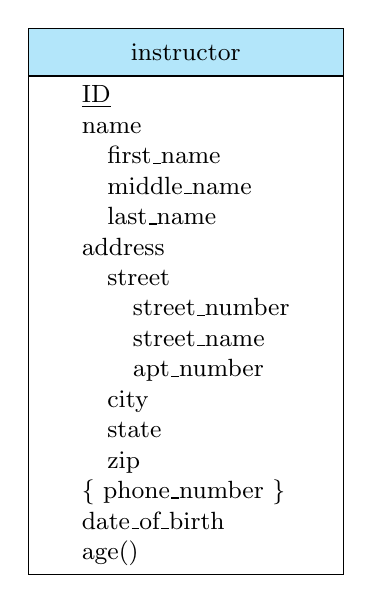
\begin{tikzpicture}[node distance=1.5cm]
    % Author table (top left)
    \node[box, fill=cyan!30, minimum height=0.6cm, minimum width=4cm] (author_header) {instructor};
    \node[box, fill=white, below=0cm of author_header.south, anchor=north, minimum height=1.2cm, minimum width=4cm] (author_body) 
    {\underline{ID} \\ name \\ \quad first\_name \\ \quad middle\_name \\ \quad last\_name \\ address \\ \quad  street \\ 
    \qquad street\_number \\ \qquad street\_name \\ \qquad apt\_number \\ \quad city \\ \quad state \\\quad zip \\ 
    \{ phone\_number \} \\ date\_of\_birth \\ age()};
\end{tikzpicture}
\begin{checkboxes} 
    \CorrectChoice 11
    \choice 14
    \choice 15
    \choice 16
    \choice 12
    \choice 13
    \choice 17
\end{checkboxes}
\end{minipage}\vspace{1em}

\begin{minipage}{\linewidth}
\question[3]
According to the E-R Diagram for a University Enterprise what should be the definition of the relation schema \textit{student}?\par\vspace{0.5em}
\begin{checkboxes}
    \choice 
    \begin{verbatim}
create table student
(ID    varchar(5), 
name varchar(20) not null, 
dept_name varchar(20), 
tot_cred numeric(3,0) check (tot_cred >= 0),
primary key (ID),
foreign key (dept_name) references department(dept_name) on delete set null
); 
    \end{verbatim}
    \CorrectChoice
    \begin{verbatim}
create table student
(ID    varchar(5), 
name varchar(20) not null, 
dept_name varchar(20), 
tot_cred numeric(3,0) check (tot_cred >= 0),
i_ID varchar(5),
primary key (ID),
foreign key (dept_name) references department(dept_name) on delete set null,
foreign key (i_ID) references instructor(ID)
);    
    \end{verbatim}
    \choice
    \begin{verbatim}
create table student
(ID    varchar(5), 
name varchar(20) not null, 
dept_name varchar(20), 
tot_cred numeric(3,0) check (tot_cred >= 0),
i_ID varchar(5) not null,
primary key (ID),
foreign key (dept_name) references department(dept_name) on delete set null,
foreign key (i_ID) references instructor(ID)
);      
    \end{verbatim}
    \choice
    \begin{verbatim}
create table instructor
(id varchar(5),
name varchar(20) not null,
dept_name varchar(20),
salary numeric(8,2),
s_ID varchar(5),
primary key(id),
foreign key (dept_name) references department(dept_name) on delete set null,
foreign key (s_ID) references student(ID)
);   
    \end{verbatim}
\end{checkboxes}
\end{minipage}\vspace{1em}

\begin{minipage}{\linewidth}
\question[3]
The school needs to track the following information: \par\vspace{0.5em}
\begin{itemize}
    \item For each student: first name, middle name, last name, phone number, and date of birth.
    \item For each instructor: first name, middle name, last name, phone number, and bank account number.
    \item For each classroom: capacity, room number, and building location.
\end{itemize}
How many entity sets will represent these requirements in the ER Model?\par\vspace{0.5em}
\begin{checkboxes} 
    \CorrectChoice 3
    \choice 4
    \choice 5
    \choice 6
\end{checkboxes}
\end{minipage}\vspace{1em}

% ------------------ MULTIPLE SELECT SECTION ------------------
\section*{Part III — Multiple select (select all that apply)}

\begin{minipage}{\linewidth}
\question[12]
How many tables will be created in the database for the model depicted in the below ER Diagram?\par\vspace{1em}
\begin{center}
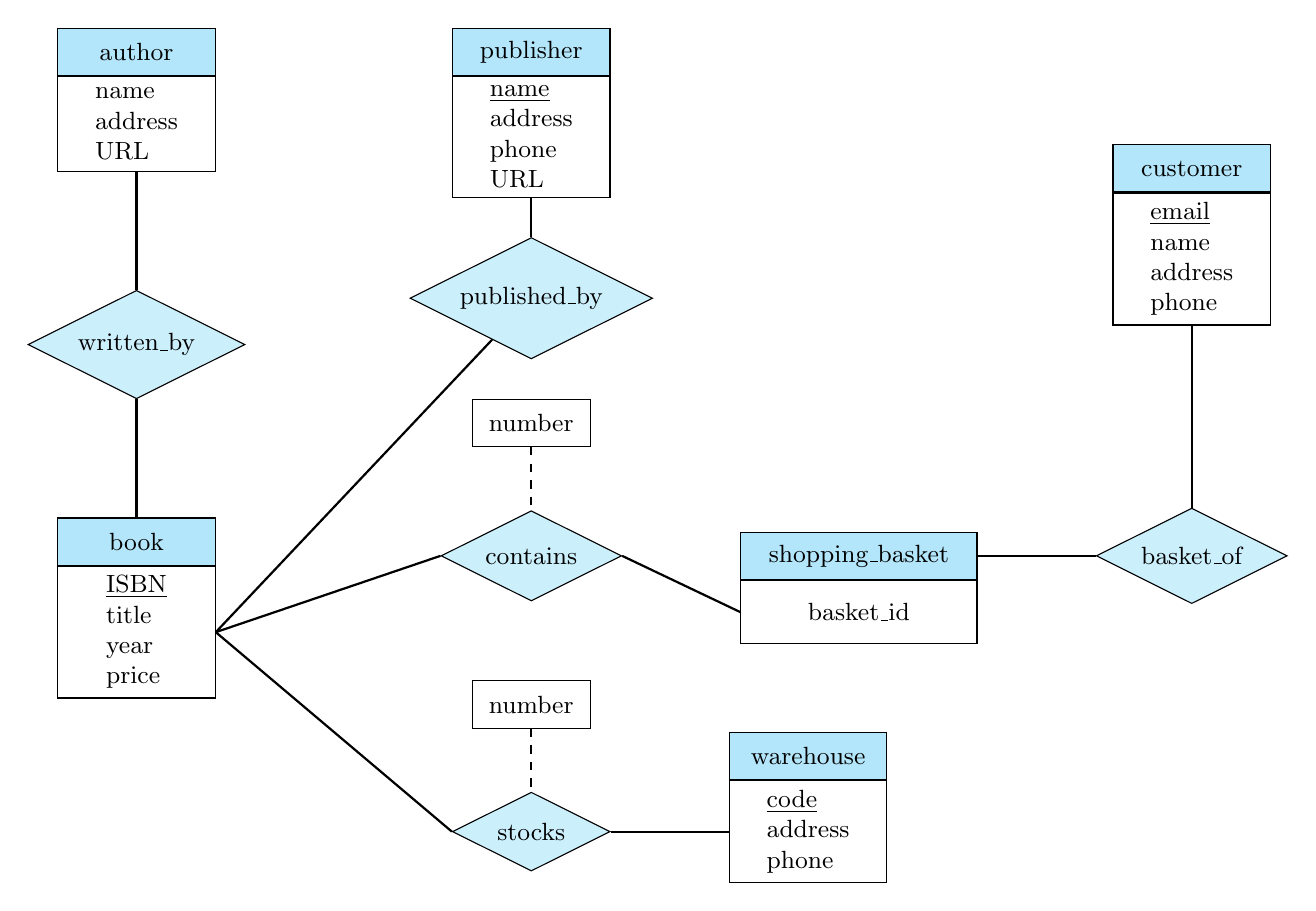
\begin{tikzpicture}[node distance=1.5cm]
    % Author table (top left)
    \node[box, fill=cyan!30, minimum height=0.6cm, minimum width=2cm] (author_header) {author};
    \node[box, fill=white, below=0cm of author_header.south, anchor=north, minimum height=1.2cm, minimum width=2cm] (author_body) {name\\address\\URL};
    
    % Written_by diamond
    \node[decision, below=1.5cm of author_body, fill=cyan!20] (written_by) {written\_by};
    
    % Book table
    \node[box, fill=cyan!30, minimum height=0.6cm, minimum width=2cm, below=1.5cm of written_by] (book_header) {book};
    \node[box, fill=white, below=0cm of book_header.south, anchor=north, minimum height=1.4cm, minimum width=2cm] (book_body) {\underline{ISBN}\\title\\year\\price};
    
    % Publisher table (top center, closer to author)
    \node[box, fill=cyan!30, minimum height=0.6cm, minimum width=2cm, right=3cm of author_header] (publisher_header) {publisher};
    \node[box, fill=white, below=0cm of publisher_header.south, anchor=north, minimum height=1.5cm, minimum width=2cm] (publisher_body) {\underline{name}\\address\\phone\\URL};
    
    % Published_by diamond
    \node[decision, below=0.5cm of publisher_body, fill=cyan!20] (published_by) {published\_by};
    
    % Number attribute for contains (top)
    \node[attribute, below=0.5cm of published_by] (number1) {number};
    
    % Contains diamond
    \node[decision, below=0.8cm of number1, fill=cyan!20] (contains) {contains};
    
    % Shopping_basket table
    \node[box, fill=cyan!30, minimum height=0.6cm, minimum width=3cm, right=1.5cm of contains] (basket_header) {shopping\_basket};
    \node[box, fill=white, below=0cm of basket_header.south, anchor=north, minimum height=0.8cm, minimum width=3cm] (basket_body) {basket\_id};
    
    % Basket_of diamond (next to shopping_basket)
    \node[decision, right=1.5cm of basket_header, fill=cyan!20] (basket_of) {basket\_of};
    
    % Customer table (above basket_of)
    \node[box, fill=cyan!30, minimum height=0.6cm, minimum width=2cm, above=4cm of basket_of] (customer_header) {customer};
    \node[box, fill=white, below=0cm of customer_header.south, anchor=north, minimum height=1.4cm, minimum width=2cm] (customer_body) {\underline{email}\\name\\address\\phone};
    
    % Number attribute for stocks (bottom)
    \node[attribute, below=1cm of contains] (number2) {number};
    
    % Stocks diamond
    \node[decision, below=0.8cm of number2, fill=cyan!20] (stocks) {stocks};
    
    % Warehouse table
    \node[box, fill=white, anchor=north, minimum height=1.2cm, minimum width=2cm, right=1.5cm of stocks] (warehouse_body) {\underline{code}\\address\\phone};
    \node[box, fill=cyan!30, above=0cm of warehouse_body.north, minimum height=0.6cm, minimum width=2cm] (warehouse_header) {warehouse};

    % Lines
    \draw[line] (author_body) -- (written_by);
    \draw[line] (written_by) -- (book_header);
    \draw[line] (publisher_body) -- (published_by);
    \draw[line] (published_by) -- (book_body.east);
    \draw[line] (book_body.east) -- (contains.west);
    \draw[dashedline] (number1) -- (contains);
    \draw[line] (contains.east) -- (basket_body.west);
    \draw[line] (customer_body) -- (basket_of);
    \draw[line] (basket_of) -- (basket_header.east);
    \draw[line] (book_body.east) -- (stocks.west);
    \draw[dashedline] (number2) -- (stocks);
    \draw[line] (stocks) -- (warehouse_body);
\end{tikzpicture}\vspace{1em}
\end{center}
\begin{checkboxes}
    \choice Attribute \textit{address} of the entity set \textit{author} is composite.
    \choice \textit{shopping\_basket} is a weak entity set.
    \CorrectChoice A book can be published by many publishers.
    \CorrectChoice Table corresponding to the relationship stocks has 3 attributes.
    \CorrectChoice There can't be two authors with the same name.
    \choice Multiple tuples can exist in the table, corresponding to the contains relationship set, 
    indicating that a particular basket contains 5 books with ISBN X. 
\end{checkboxes}
\end{minipage}\vspace{1em}

\begin{minipage}{\linewidth}
\question[8]
What is true about the below diagram?\par\vspace{0.5em}
\begin{center}
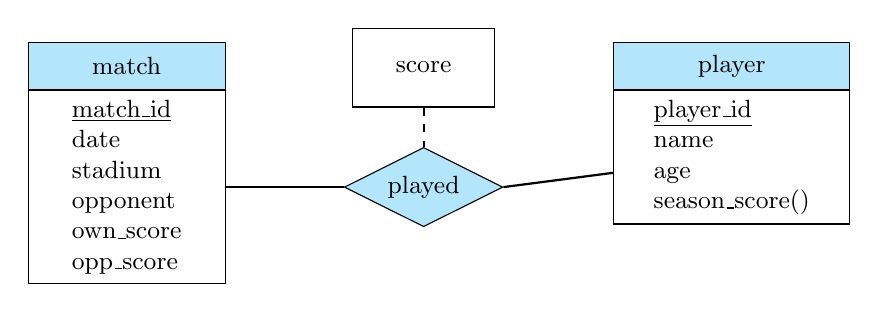
\begin{tikzpicture}[node distance=1.5cm]
    % match table
    \node[box, fill=cyan!30, minimum height=0.6cm, minimum width=2.5cm] (match_header) {match};
    \node[box, fill=white, below=0cm of match_header.south, anchor=north, minimum height=1cm, minimum width=2.5cm] (match_body) {\underline{match\_id}\\date\\stadium\\opponent\\own\_score\\opp\_score};

    % played diamond
    \node[decision, fill=cyan!30, right=1.5cm of match_body, inner sep=0.09cm] (played) {played};

    % Score box
    \node[box, fill=white, above=0.5cm of played] (score) {score};

    % player table
    \node[box, fill=cyan!30, minimum height=0.6cm, minimum width=3cm, right=1.5cm of score] (player_header) at (score.east |- match_header) {player};
    \node[box, fill=white, below=0cm of player_header.south, anchor=north, minimum height=1cm, minimum width=3cm] (player_body) {\underline{player\_id}\\name\\age\\season\_score()};
    
    % Lines
    \draw[line] (match_body) -- (played);
    \draw[dashedline] (score) -- (played);
    \draw[line] (played.east) -- (player_body);
\end{tikzpicture}\vspace{1em}
\end{center}
(Select all that apply)\par\vspace{0.5em}
\begin{checkboxes}
    \CorrectChoice \textit{season\_score} is a derived attribute
    \CorrectChoice On a given day, it's possible for two distinct matches to take place at the same stadium.
    \CorrectChoice The attribute \textit{age} can potentially contain outdated (stale) information. 
    \CorrectChoice No players can play in a match.
\end{checkboxes}
\end{minipage}\vspace{1em}

\begin{minipage}{\linewidth}
\question[8]
What is true about the below diagram?\par
(Select all that apply.)\par\vspace{1em}
\begin{center}
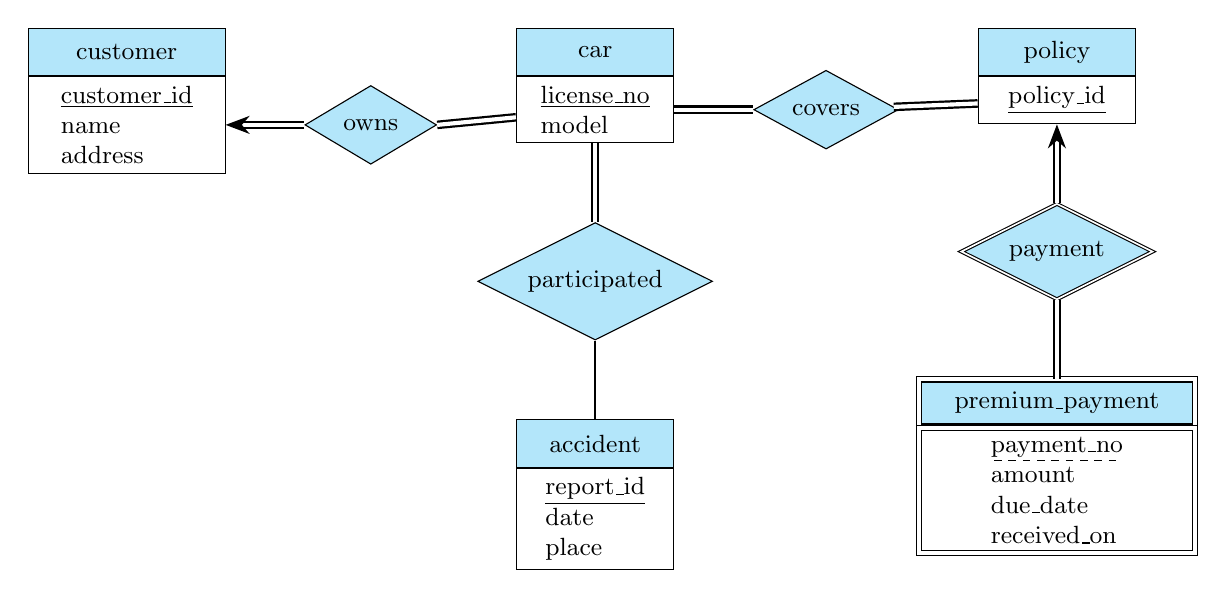
\begin{tikzpicture}[node distance=2cm]
    % Customer table
    \node[box, fill=cyan!30, minimum height=0.6cm, minimum width=2.5cm] (customer_header) {customer};
    \node[box, fill=white, below=0cm of customer_header.south, anchor=north, minimum height=1.2cm, minimum width=2.5cm] (customer_body) {\underline{customer\_id}\\name\\address};
    
    % Owns diamond
    \node[decision, fill=cyan!30, right=1cm of customer_body] (owns) {owns};
    
    % Car table
    \node[box, fill=cyan!30, minimum height=0.6cm, minimum width=2cm, right=1cm of owns] (car_header) at (owns.east |- customer_header) {car};
    \node[box, fill=white, below=0cm of car_header.south, anchor=north, minimum height=0.8cm, minimum width=2cm] (car_body) {\underline{license\_no}\\model};
    
    % Covers diamond
    \node[decision, fill=cyan!30, right=1cm of car_body] (covers) {covers};
    
    % Policy table
    \node[box, fill=cyan!30, minimum height=0.6cm, minimum width=2cm, right=1cm of covers] (policy_header) at (covers.east |- car_header) {policy};
    \node[box, fill=white, below=0cm of policy_header.south, anchor=north, minimum height=0.6cm, minimum width=2cm] (policy_body) {\underline{policy\_id}};
    
    % Participated diamond
    \node[decision, fill=cyan!30, below=1cm of car_body] (participated) {participated};
    
    % Accident table
    \node[box, fill=cyan!30, minimum height=0.6cm, minimum width=2cm, below=1cm of participated] (accident_header) {accident};
    \node[box, fill=white, below=0cm of accident_header.south, anchor=north, minimum height=1.2cm, minimum width=2cm] (accident_body) {\underline{report\_id}\\date\\place};
    
    % Payment diamond (double border)
    \node[doubledecision, fill=cyan!30, below=1cm of policy_body] (payment) {payment};
    
    % Premium_payment table (double border)
    \node[doublebox, fill=cyan!30, minimum height=0.6cm, minimum width=3.5cm, below=1cm of payment] (premium_header) {premium\_payment};
    \node[doublebox, fill=white, below=0cm of premium_header.south, anchor=north, minimum height=1.4cm, minimum width=3.5cm] (premium_body) {\dashuline{payment\_no}\\amount\\due\_date\\received\_on};
    
    % Lines and arrows
    \draw[doublearrow] (owns) -- (customer_body);
    \draw[doubleline] (owns.east) -- (car_body);
    \draw[doubleline] (car_body) -- (covers);
    \draw[doubleline] (covers) -- (policy_body);
    \draw[doubleline] (car_body) -- (participated);
    \draw[line] (participated) -- (accident_header);
    \draw[doublearrow] (payment) -- (policy_body);
    \draw[doubleline] (payment) -- (premium_header);
    
\end{tikzpicture}
\end{center}
\begin{checkboxes}
    \CorrectChoice A customer can own many cars.
    \CorrectChoice A car needs to participate in at least one accident.
    \choice 5 tables will be created in the database.
    \choice \textit{premium\_payment} table will have a primary key consisting of one attribute.
\end{checkboxes}
\end{minipage}\vspace{1em}

\begin{minipage}{\linewidth}
\question[4]
\textit{Instructor} relation references \textit{department} relation. If the foreign key constraint was removed from the \textit{instructor} table, 
for which event(s) trigger(s) would have to be implemented to ensure that the \textit{dept\_name} values in the \textit{instructor} table align 
with valid entries in the \textit{dept\_name} attribute of the \textit{department} table?\par\vspace{0.5em}
\begin{checkboxes} 
    \CorrectChoice insert on \textit{instructor}
    \choice insert on \textit{department}
    \CorrectChoice update on \textit{instructor}
    \CorrectChoice update on \textit{depertment}
    \choice delete from \textit{instructor}
    \CorrectChoice delete from \textit{department}
\end{checkboxes}
\end{minipage}\vspace{1em}

\begin{minipage}{\linewidth}
\question[8]
What is true about the below diagram?\par\vspace{0.5em}
\begin{center}
\begin{tikzpicture}[node distance=1.5cm]
    % instructor table
    \node[box, fill=cyan!30, minimum height=0.6cm, minimum width=2.5cm] (instructor_header) {instructor};
    \node[box, fill=white, below=0cm of instructor_header.south, anchor=north, minimum height=1cm, minimum width=2.5cm] (instructor_body) {\underline{ID}\\name\\salary};

    % advisor diamond
    \node[decision, fill=cyan!30, right=1.5cm of instructor_body, inner sep=0.09cm] (advisor) {advisor};

    % date box
    \node[box, fill=white, above=0.5cm of advisor] (date) {date};

    % student table
    \node[box, fill=cyan!30, minimum height=0.6cm, minimum width=3cm, right=1.5cm of score] (student_header) at (date.east |- instructor_header) {student};
    \node[box, fill=white, below=0cm of student_header.south, anchor=north, minimum height=1cm, minimum width=3cm] (student_body) {\underline{ID}\\name\\tot\_cred};
    
    % Lines
    \draw[line] (instructor_body) -- (advisor);
    \draw[dashedline] (advisor) -- (date);
    \draw[line] (advisor.east) -- (student_body);
\end{tikzpicture}\vspace{1em}
\end{center}
(Select all that apply)\par\vspace{0.5em}
\begin{checkboxes}
    \choice \textit{advisor} is of type one-to-one.
    \choice Table corresponding to the \textit{student} entity set will have a foreign key, because of the 
        \textit{advisor} relationship \textit{student} participates in.
    \CorrectChoice A student may have zero, one, or multiple advisors. 
    \choice Table corresponding to the \textit{instructor} entity set will have a foreign key, 
    because of the \textit{advisor} relationship \textit{instructor} participates in.
\end{checkboxes}
\end{minipage}\vspace{1em}

% ------------------ Fill In The Blank SECTION ------------------
\section*{Part IV — Fill In The Blank}

\begin{minipage}{\linewidth}
\question[2]
Based on the "\textbf{E-R Diagram for a University Enterprise}" relation corresponding to the \textit{sec\_time\_slot} relationship should have
 \ifprintanswers\textbf{2/two }\else\fillin[][8em]\fi foreign key(s).
\end{minipage}\vspace{1em}

\end{questions}
\end{document}